\documentclass[english]{article}
\usepackage[T1]{fontenc}
\usepackage[utf8]{inputenc}
\usepackage{geometry}
\geometry{verbose,tmargin=3.5cm,bmargin=4cm,lmargin=3.8cm,rmargin=3.8cm}

% plots
\usepackage{graphicx}
\graphicspath{ {../plots/} }
\usepackage{calc}
% state diagrams
\usepackage{tikz}
\usetikzlibrary{automata, positioning, arrows}
\tikzset{
  initial text={},
  ->, % makes the edges directed
  node distance=3.5cm, % specifies the minimum distance between two nodes. Change if necessary.
  every state/.style={rectangle, thick, text width=5em, align=center}  % sets the properties for each ’state’ node
}

% tables
\usepackage{multirow}
% quotation
\usepackage{dirtytalk}

% import natbib and sets bibliography and citation styles
\usepackage[numbers,sort]{natbib}
\bibliographystyle{apalike}

\makeatletter
\usepackage{hyperref}

\makeatother
\usepackage{babel}

% % work in progress packages
% \newcommand{\citationneeded}{\textsuperscript{\color{blue} [citation needed]}}
% \usepackage{easy-todo}

\begin{document}

% \listoftodos

\title{Keep your enemies closer and be loud about it}
\author{
  Martin Toman; TUDelft
  \\
  m.toman@student.tudelft.nl
\and
  Dr. Neil Yorke-Smith; TUDelft
  \\
  n.yorke-smith@tudelft.nl
}
\date{20 June 2021}
\maketitle


\begin{abstract}
% The abstract should be short and give the overall idea:
% what is the background, the research questions, what is contribution, and what are the main conclusions.
% It should be readable as a stand-alone text (preferably no references to the paper or outside literature).

Under what conditions can cooperation emerge and how can we sustain it?
We build a computer simulation of a multi-agent spatial environment using Prisoner's Dilemma as the principal agent interaction.
We expand the model by allowing agents to remember a fixed number of past defectors
and abstain from interacting with them again.
Agents will be allowed to communicate by openly announcing remembered defectors, warning nearby agents.
This way local reputation of each agent is created.
We measure how well our model sustains cooperation and how robust it is against environmental harshness.
The conclusion we reach is that local reputation works excellent in sustaining cooperation and punishing defection.
The length of agent memory and amount of gossip are not important factors,
only the range of gossip has to be greater than the agent movement speed.

\end{abstract}



\section{Introduction}

% intro - what is prisoner's dilemma
How can we encourage and sustain cooperation? Humans dominate their environments thanks to our ability to cooperate flexibly and at scale, as argued by \citet{harari-sapiens}.
To study the conditions necessary for cooperation to flourish we need a suitable model of an activity with temptations to defect and punishments for doing so.

In 1950, Albert Tucker named a two-player exchange game
\say{the Prisoner's Dilemma} to attract more research interest \citep{sep-prisoner-dilemma}.
This game elegantly captures the difficulty of the decision between cooperation and defection in a single choice.
Despite being so simple compared to the complexity of the problem it is representing, it was used to model many aspects of behaviour in systems of selfish individuals; and, according to \citet{Axelrod84}, for \say{discovery of the precise conditions that are necessary and sufficient for cooperation to emerge}.

% iterated version + the dilemma
In the case of a one-off exchange, there being no opportunity for a follow-up punishment, the rational behaviour is defection. (This extends to all rounds for a fixed-length game, inductively \citep{Axelrod84}.)
The interesting behaviour arises if there is no end; or, at least, if there is no way for the participants of the game to know when the game ends or even if there is an end.
% reputation importance
An agents has to expect that even a single defection can be infinitely punished by never again being cooperated with \citep{GRIM}.
Such a risk may just not be worth it.

% global reputation system
The defectors can, naturally, only be punished if they can be identified and known to others. This is why services like Ebay or Airbnb have a rating system in place.
Presence of a reputation system strongly boosts cooperation, as shown by \citet{simple-reputation, public-private-monitoring}.
These studies used groups of volunteers as game participants and explored the effects of various information being public - from only the latest move of the current opponent, to full histories of all moves taken by every participant.

% decentralizing reputation: keeping track internally?
Using human subjects as game participants limited the research to relatively small groups with few rounds; they also used external infrastructure for information passing: eliminating noise, delays, and deliberately wrong information.
As shown by \citet{noise}, not all strategies that perform well in noise-less environments can do so under the presence of noise.

Using external infrastructure for passing information also meant that the transmission speed was uniform for all participants receiving all necessary information in time for their next round of the game.
These are non-trivial idealizations: relaxing them would yield a model closer to real-world systems and could change the results dramatically.

In this paper we aim to find out if, and how well, can local reputation sustain cooperation and under what parameters does it yield optimal results.
We evaluate the approach under various gossip range and memory length; and comment on the effectiveness of local reputation in enforcing cooperation in spatial prisoner's dilemma.

In the next section we define the goals explicitly and show the methodology we will use for this research.
Afterwards we show the results with short impartial explanations, followed by discussion of the implications of the results obtained;
we also connect our results with similar research.
We close the paper with a short reflection on the ethical aspects and the reproducibility of this paper,
after which we summarize and explicitly state our conclusions with some ideas for further research directions.


\section{Methodology}
We aim to measure the effectiveness of local reputation in enforcing cooperation.
To do this we will build a computer simulation of a multi-agent spatial environment.
We will use a Spatial Iterated Prisoner's Dilemma as the principal exchange game for modelling agent interactions.
We hypothesize that local reputation will drive the simulation towards a cooperator-only population and will be able to sustain it indefinitely.

In this section we define the goals of this paper explicitly,
explain the design of the model and simulations,
and present the measurable properties and evaluation criteria of the model.
We end the section with an explanation of how we will connect our simulation results back to the original question
and what would constitute a confirmation of our hypothesis.

\subsection{Problem Statement}
We will use the prisoner's dilemma game to model agent interactions.
This is a good choice for modelling behaviour of rational and selfish actors.
And will allow us to observe the conditions necessary for cooperation to emerge in the population as well as what makes it sustain itself.

The agents will live in a spatial environment and act independently;
the only mutual interactions will be playing the PD game with a neighbor and exchanging gossip with nearby agents.
We will vary the range at which the gossip can be exchanges as well as the amount of information which can be included in a single gossip message.
We want to determine the effectiveness of the gossip mechanism in promoting and sustaining cooperation.

\subsection{Simulation Design}
% Typically in general research articles, the second section contains a description of the research methodology, explaining what you, the researcher, is doing to answer the research question(s), and why you have chosen this method.
% This section includes references to necessary background information.

To explore the effects of local reputation, built up via openly gossiping with nearby neighbors,
we will use a computer simulation of a multi-agent spatial environment.
We will base the simulation on the design of \citet{smaldino}.

\begin{figure}[h]
  \centering
  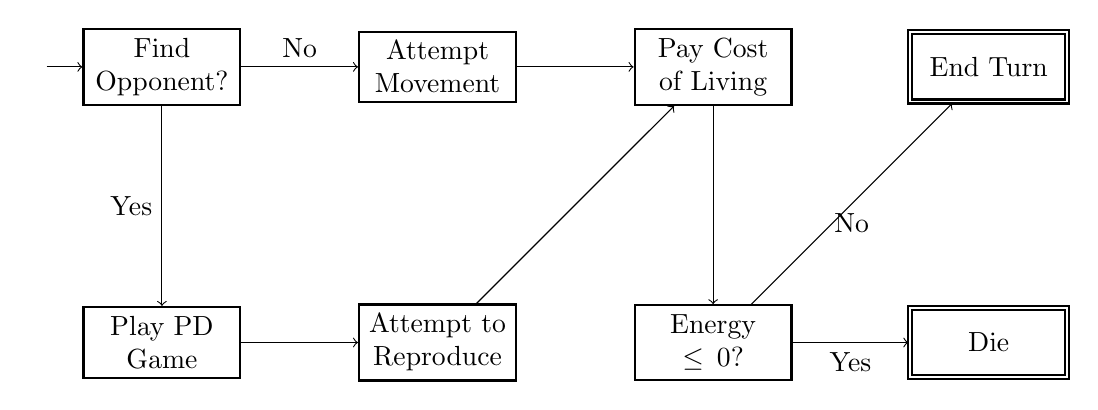
\begin{tikzpicture}

    \node[state, initial] (find_opponent) {Find Opponent?};

    \node[state, below of=find_opponent] (play) {Play PD Game};
    \node[state, right of=play] (reproduce) {Attempt to Reproduce};
    \node[state, right of=find_opponent] (move) {Attempt Movement};
    \node[state, right of=move] (cost) {Pay Cost of Living};
    \node[state, below of=cost] (energy) {Energy $\le 0$?};

    \node[state, accepting, right of=energy] (die) {Die};
    \node[state, accepting, above of=die] (end) {End Turn};

    \draw
      (find_opponent) edge[left] node{Yes} (play)
      (find_opponent) edge[above] node{No}  (move)
      (play) edge[] node{} (reproduce)
      (reproduce) edge[] node{} (cost)
      (move) edge[] node{} (cost)
      (cost) edge[] node{} (energy)
      (energy) edge[below] node{No}  (end)
      (energy) edge[below] node{Yes} (die)
      ;
  \end{tikzpicture}
  \caption{Agent behaviour diagram: showing the decision flow of an agent's single turn}
  \label{fig:agent_behaviour}
\end{figure}

The model consists of a spatial environment:
square grid with torus (wrapping) bounds,
each cell can be occupied by a single agent.
This is a discreet time model;
at each time step, every agent takes a single turn.
The order in which agents take their turn is randomized in each time step.
Agent's turn is defined by the finite state diagram shown in Figure \ref{fig:agent_behaviour}.
The agents pay a fixed cost to survive ($k = 0.5$) to the next round (agents who deplete their energy die and are removed from the simulation), and try to reproduce once they accumulate enough energy via positive interactions with other agents - PD game wins.

Every agent can play at most a single PD game in each time step.
Playing a game in a time step is not guaranteed and depends on the spatial configuration of agents, order in which the agents are scheduled, and randomness in choosing an opponent from agent's neighbors.
Similarly, when no opponent is found, movement only happens if an empty cell is found nearby; if there is more than one empty cell, one is chosen at random.

Agents reproduce by creating a new agent with the same parameters as themselves in an empty neighborhood cell (chosen randomly if more than one, no reproduction if there are no empty cells in the neighborhood).
Reproduction is only attempted if the agent has accumulated enough energy: at least twice the amount of the cost of reproduction.
The cost of reproduction is then subtracted from the parent and the offspring is birthed with this energy level.
The cost of reproduction is effectively transferred from the parent to the offspring;
reproducing does not change the net amount of energy in the model.

\begin{table}[h!]
  \centering
  \begin{tabular}{c c||c|c}
    & & \multicolumn{2}{c}{Opponent's move} \\
    & & Cooperate & Defect \\
    \hline\hline

    \multirow{4}{6em}{Player's move}
    & \multirow{2}{5em}{Cooperate}
      & Player:\ \ \ \ \ \ R & Player:\ \ \ \ \ \ S \\
    & & Opponent: R & Opponent: T \\
    \cline{2-4}
    & \multirow{2}{5em}{Defect}
      & Player:\ \ \ \ \ \ T & Player:\ \ \ \ \ \ P \\
    & & Opponent: S & Opponent: P \\
  \end{tabular}

  \caption{Payoff matrix}
  \label{table:payoff}
\end{table}

A single round of the game is defined using a payoff matrix as shown in Table \ref{table:payoff}, with $T > R > P > S$ and $2R > T + S$ \citep{chammah1965}.
Like in the original model \citep{smaldino},
we use $R = 3$ (reward for cooperating),
$T = 5$ (temptation to defect),
$P = 0$ (punishment for mutual defection).
We use a different $S = -1.5$ (sucker's payoff - cooperator got defected) from $S = -1.0$ in the original.

We choose the sucker's payoff value ($S = -1.5$) empirically,
by running simulations of the model and taking note of a value which leads to cooperator extinction relatively quickly.
This choice for the parameter will ensure that, if we reach cooperation, it was caused by the reputation mechanism;
and not because of random interactions in the model.

Environmental harshness of the model is defined by
the sucker's payoff $S$ (social harshness) and
the cost to survive $k$ (external harshness).
We will investigate the effect of varying these parameters on our results
and check the robustness of gossip in promoting cooperation across environments of various harshness.

To better suit our needs we will introduce some changes to the original model.
We will reduce the spatial grid size from 100x100, as in the original design, to a more manageable 20x20.
This will allow us to run more simulations with more complex agent behaviour in a reasonable amount of time.
We will also decrease the starting number of agents from 1600 to 64: keeping the same percentage of 16\% of the total grid size occupied as in the original model.

This reduction of the environment size (by a factor of 25!) has the effect of significantly increasing the chance of a total extinction of all agents:
caused by the random behaviour of agents exploiting each other until all cooperators are dead and the population of pure defectors cannot sustain itself.
We disregard runs that end in extinction and increase the number of simulation runs to compensate for this.

We will expand the model by giving the agents a (limited size) memory to keep track of past defectors and later to allow them to actively and freely share this knowledge by gossiping with other agents in a given range.
Prior research \citep{memory, reciprocity, adaptive-interaction} has already shown that memory can be an effective tool in promoting cooperation.

Another expansion to the model will be the addition of the localized gossip mechanism.
This will allow agents to consult nearby peers to try and find out the reputation of agents unknown to the agents themselves.
The range at which agents can be contacted and the amount of information which agents provide will be varied.
In the results section, an overview of the effects of varying the parameters of the gossip is shown.
We believe this extension of the model will have a strong positive effect on sustaining cooperation in the model.

The simulation will be implemented in Python using the Mesa\footnote{\url{https://github.com/projectmesa/mesa}} framework.

\subsection{Simulation Evaluation}

To determine the effectives of gossip in promoting cooperation, we will observe the rate of convergence to a population of cooperators, stopping the simulation once stable equilibrium is achieved.
To verify that this is indeed an equilibrium, we let the simulation run longer and check that the general behaviour does not change after some point:
we assume that if the behaviour of the simulation only varied in the first 5\% of the  simulation and then remained unchanged, it has converged.
We will also observe the maximal population size of defectors which can sustain itself alongside the cooperators.

The main properties measured about the model will be the saturation of cooperator and defector populations.
We will measure the saturation as the fraction of agents of the type alive in the model divided by
the total carrying capacity of the population: 50\% of all the cells.
This differs from the measure of agent type frequency used by \citet{smaldino};
we have chosen to use the saturation measurement because with the decreased size model we encounter total extinction more often,
and with the gossip extension aim to speed up defector extinction.

We believe the measure of agent type saturation is clearer and easier to understand
as the relative population sizes do not influence the measure of the other type (as frequency does).
Consider the case of 10 defector and 10 cooperator with maximal carrying capacity of 20 for either type:
saturation is 50\% for both agent types, and cooperator frequency is also 50\%.
Now 10 more cooperators are born:
defector saturation stays at 50\%, cooperator saturation increases to 100\%,
but the cooperator frequency is now at 33.3\%.
Using the saturations explains what happened more clearly, at the cost of having to present 2 complementary charts for each measurement:
one for cooperator and one for defector saturation.

Since we are simulating stochastic behaviour and we are interested in the converged outcomes,
we will run every simulations 30 times for each parameter combination and we will plot the standard deviations of the results.
We will drop the 2 most extreme outliers, both positive and negative, from the plots; this allows us to show the actual behaviour of the model, devoid of unusual probabilistic anomalies.
To ensure integrity of the results, we check the outliers removed and investigate any unusual interactions for relevance to the results.

We will also record characteristic patterns formed by the populations as influenced by different parameters.
We do this, because it was shown by earlier work \citep{spatial-patterns} that in Spatial Prisoner's Dilemma interesting patterns can emerge over time.
These patterns are very similar to patterns occurring in nature, which are often created by reaction-diffusion processes.
This suggests a deeper link between our model and biological activity.



\section{Results}
Now we present the results of our simulation
with commentary on the setup and the meaning of the results.
We show the results impartially and let the data do most of the talking.
A thorough explanation of the data in the context of similar research
with explanation of wider implications will be in the next section.

We start by presenting the behaviour of the baseline (no memory, no gossip) model in the first subsection,
then we expand it by adding memory and show how this alters the results obtained,
afterwards we enable communication (gossip) between agents and run the simulation once again.

After making the comparisons between the behaviour as influenced by various extensions we take a closer look at the robustness of the gossip model against environmental harshness: both social (sucker's payoff $S$) and external (cost of living $k$).

We end this section by comparing the characteristic spatial patterns of the models.
This can provide some intuition behind the behaviour of the various models and
could be a good starting point for readers less familiar with the topic.


\subsection{Baseline model}
First we look at the plain model with 0-memory and no communication (gossip) between agents.
This is a replication of \citet{smaldino}; with some alterations.
As explained in the model design subsection, we modify the original model slightly.
We decrease the size of the grid from 100x100 to 20x20,
and decrease the starting agent count from 1600 to 64.
We will keep the following parameters unchanged:
starting energy will be randomly chosen for each agent to be between 1 and 49 (inclusive),
energy cost to reproduce is 50 (agent has to accumulate at least 100 energy and reproduces by transferring 50 to the offspring),
and the maximum energy an agent can hold is 150.

For the PD game payoffs we will use $R = 3$, $T = 5$, $P = 0$,
and for the living cost $k = 0.5$.
These values were shown to lead to the cooperators struggling to survive
and maintain their numbers \citep{smaldino}.
We will determine the value for $S$ (sucker's payoff) from the simulations.
Unless otherwise noted, we will use these parameters for all simulation runs.

\begin{figure}[!ht]
  \centering
  \makebox[\textwidth]{
    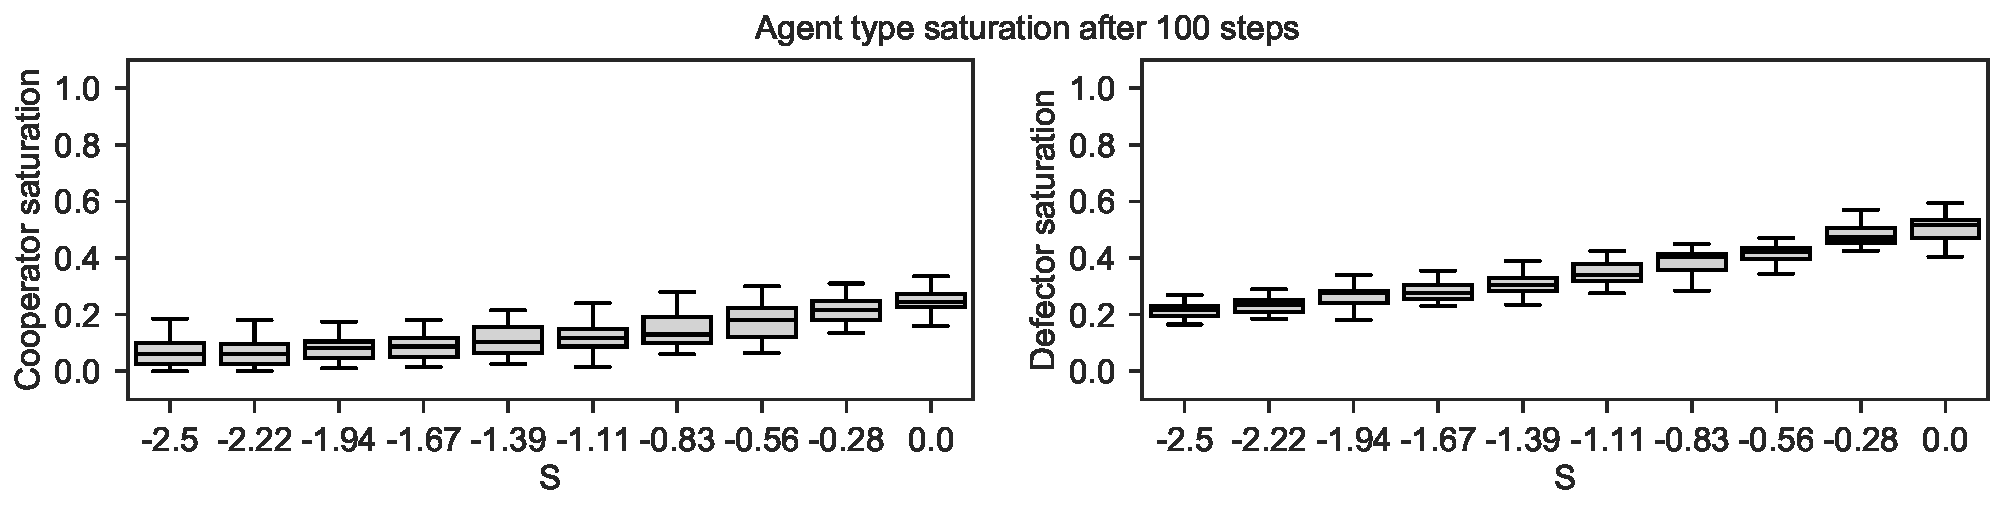
\includegraphics[width=\paperwidth-4cm]{saturation&S-memory0+gossip0_100steps_large}
  }
  \makebox[\textwidth]{
    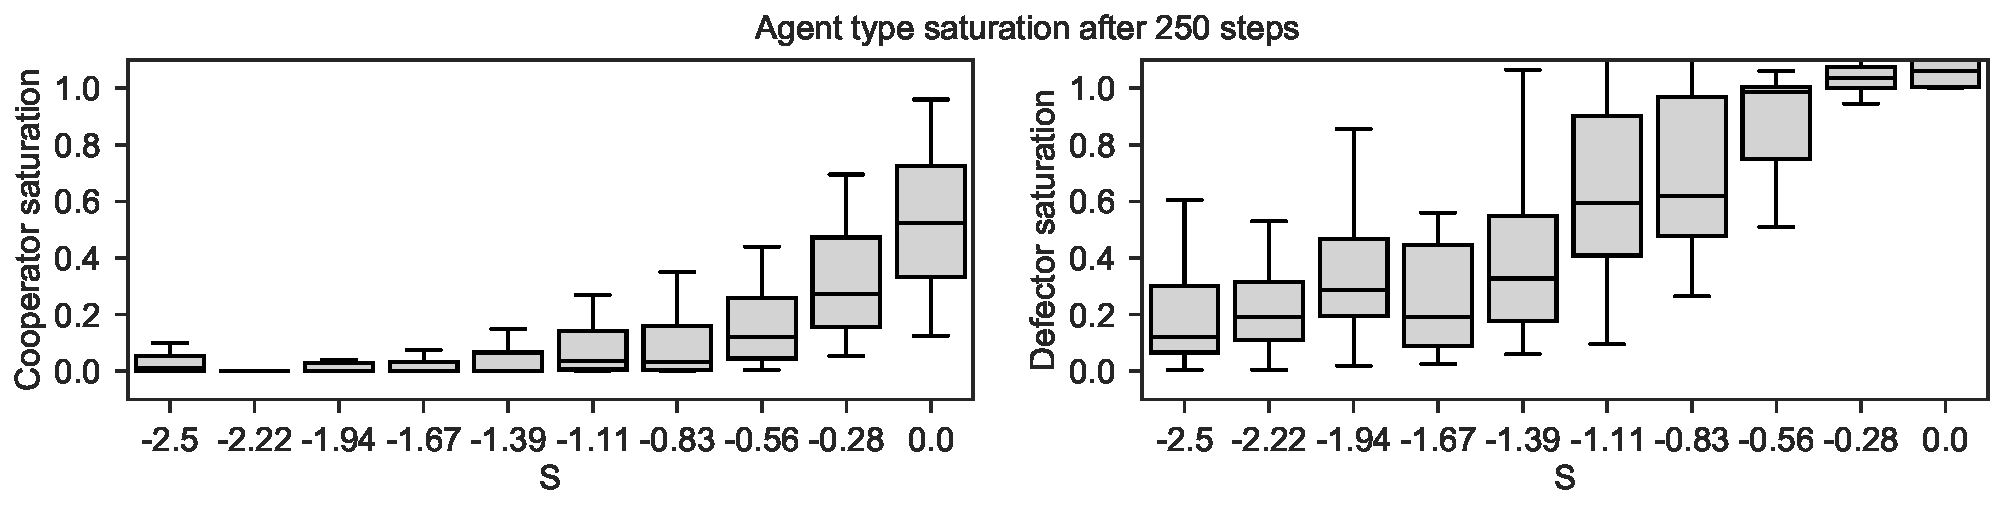
\includegraphics[width=\paperwidth-4cm]{saturation&S-memory0+gossip0_250steps_large}
  }
  \makebox[\textwidth]{
    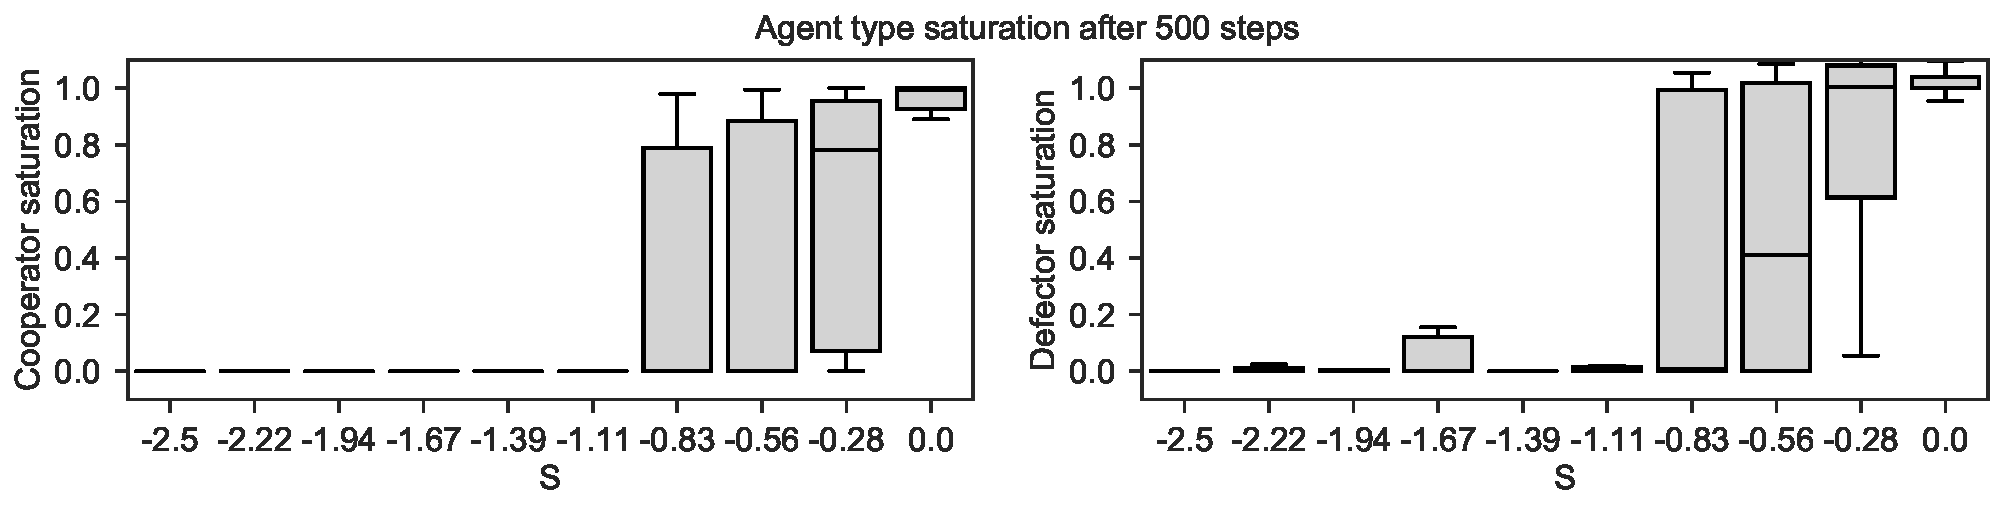
\includegraphics[width=\paperwidth-4cm]{saturation&S-memory0+gossip0_500steps_large}
  }
  \makebox[\textwidth]{
    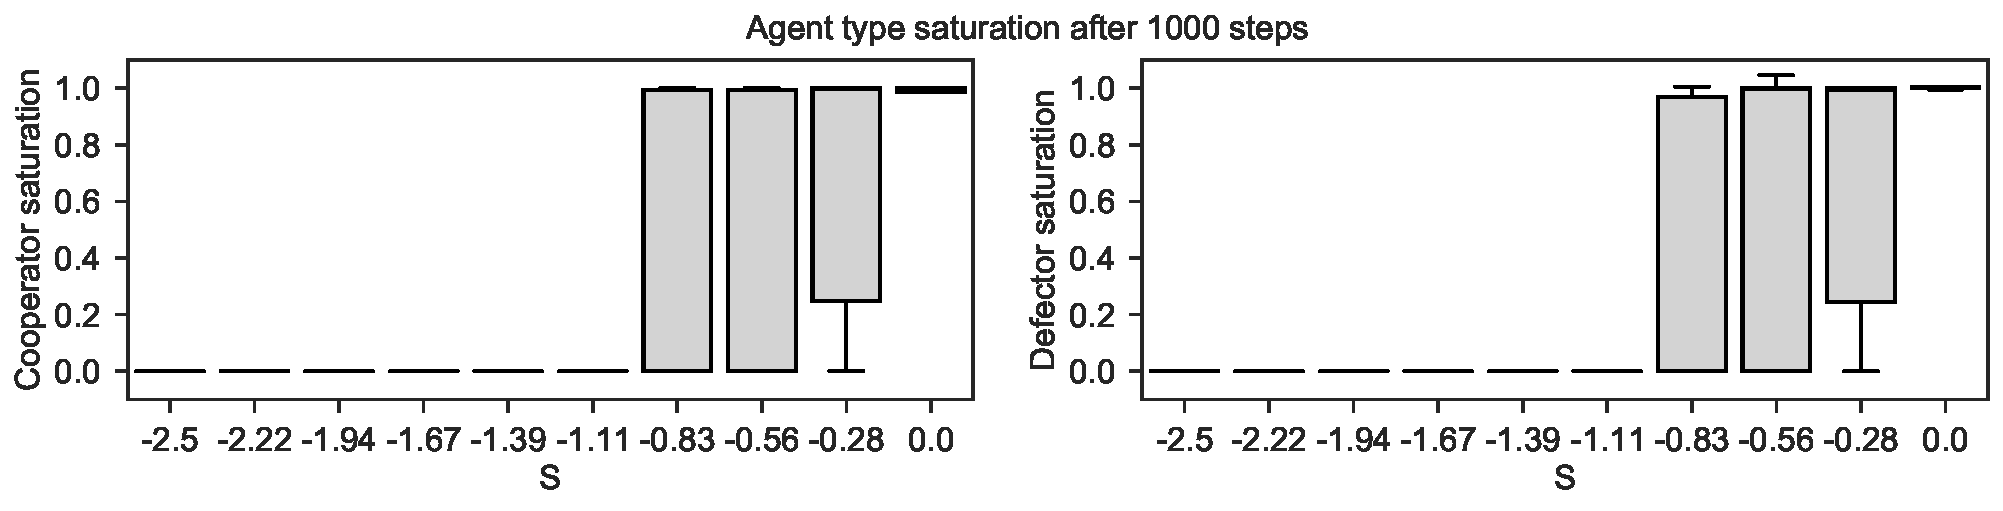
\includegraphics[width=\paperwidth-4cm]{saturation&S-memory0+gossip0_1000steps_large}
  }
  \caption{Agent type saturation for various $S$ (sucker's payoff) after 100, 250, 500, 1000 steps; SD of 30 simulation runs, outliers removed}
  \label{fig:agent_sat/S-memory0gossip0}
\end{figure}

We begin by exploring the robustness of the model against social harshness - represented by the $S$ (sucker's payoff) parameter.
In Figure \ref{fig:agent_sat/S-memory0gossip0} we present the results of running the simulation for $2.5 \leq S \leq 0.0$.
We observe that $S = -1.5$ leads to total extinction in the model by step 500;
we will use this value for the parameter for further simulations to determine the effectiveness of memory and the gossip mechanism at promoting and sustaining cooperation.


\subsection{Remember defectors}
\begin{figure}[!ht]
  \centering
  \makebox[\textwidth]{
    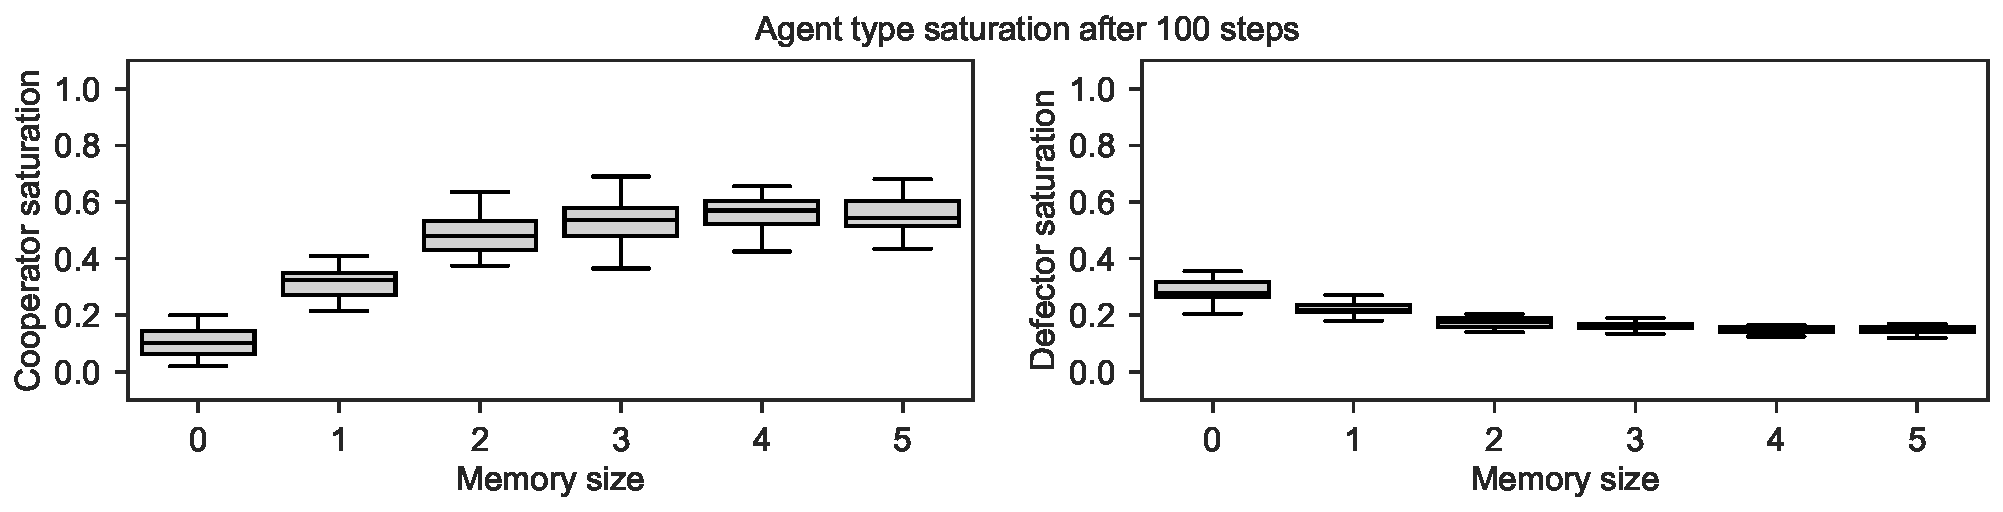
\includegraphics[width=\paperwidth-4cm]{saturation&memory_size-gossip0_100steps_large}
  }
  \makebox[\textwidth]{
    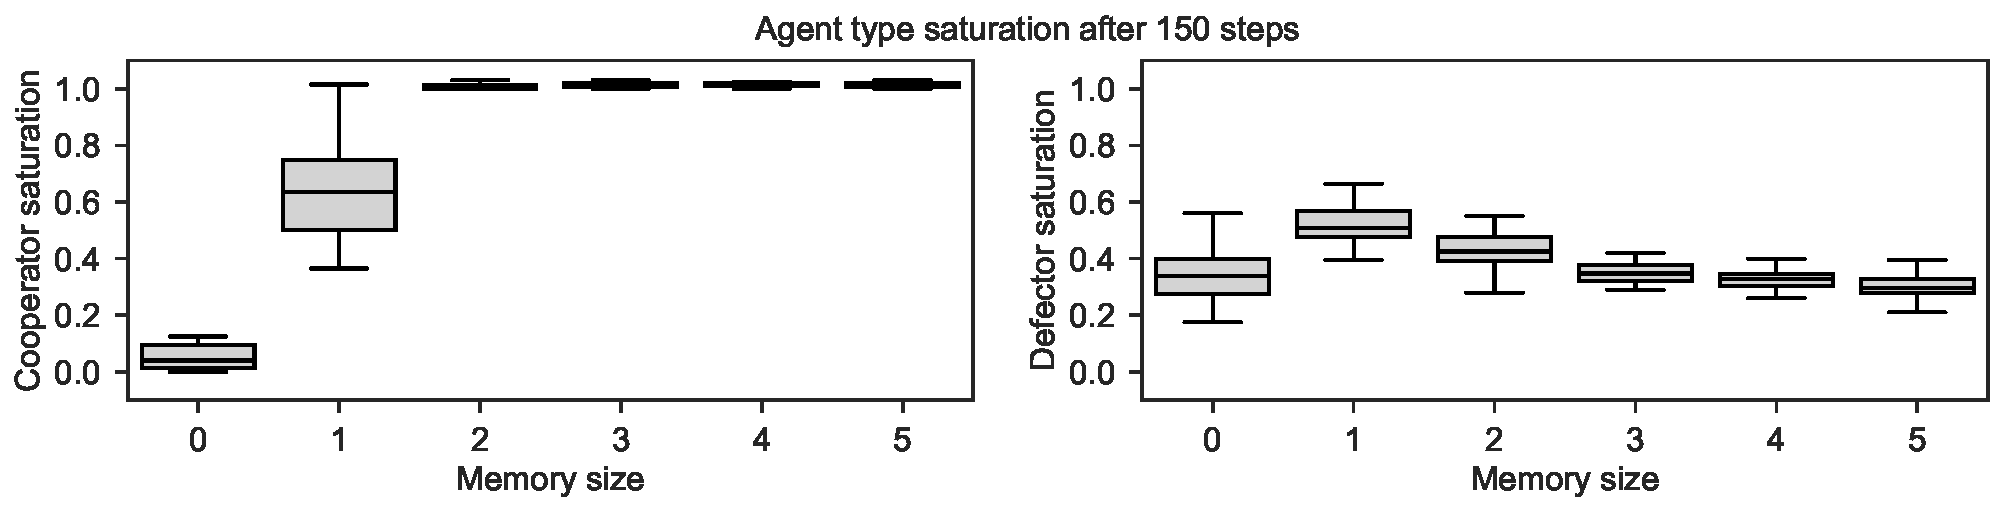
\includegraphics[width=\paperwidth-4cm]{saturation&memory_size-gossip0_150steps_large}
  }
  \makebox[\textwidth]{
    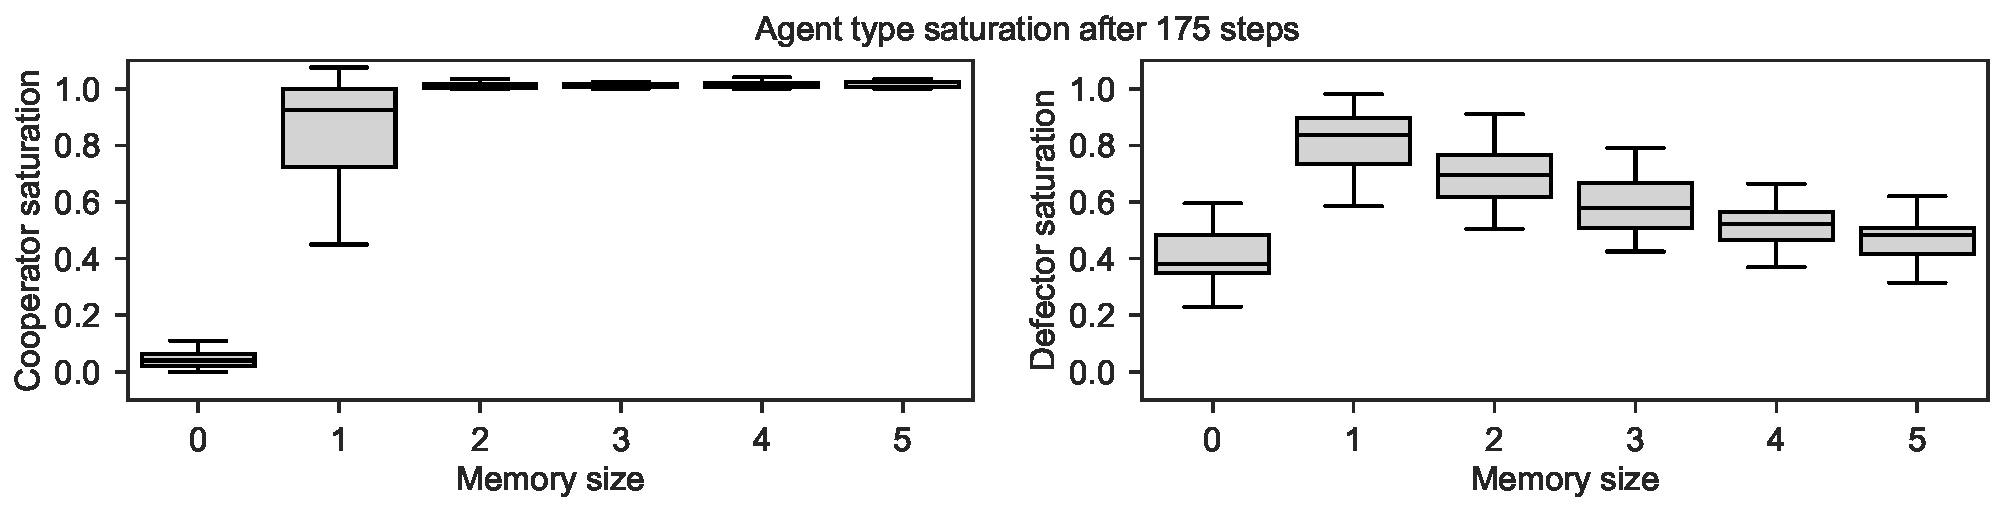
\includegraphics[width=\paperwidth-4cm]{saturation&memory_size-gossip0_175steps_large}
  }
  \makebox[\textwidth]{
    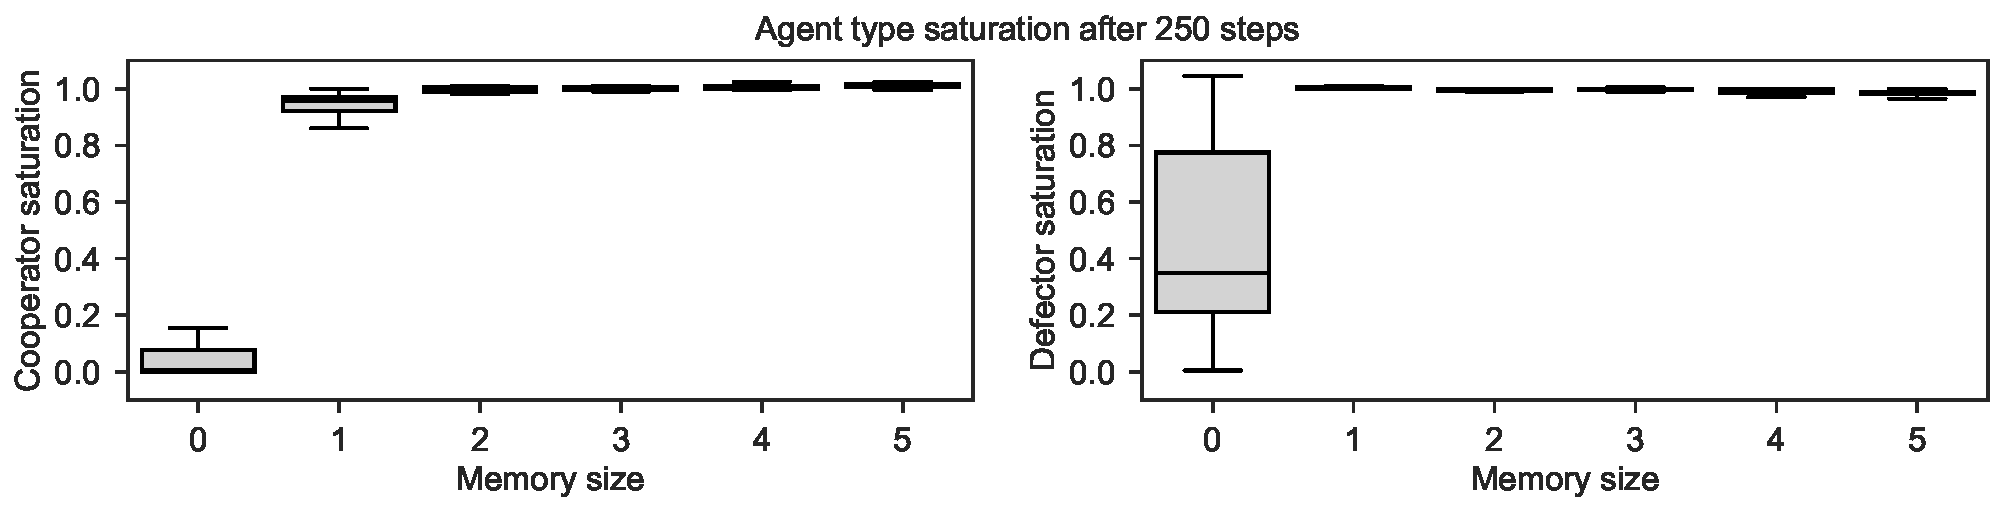
\includegraphics[width=\paperwidth-4cm]{saturation&memory_size-gossip0_250steps_large.pdf}
  }
  \caption{Agent type saturation for various memory sizes after 100, 150, 175, 250 steps; SD of 30 simulation runs, outliers removed}
  \label{fig:agent_sat/memory_size}
\end{figure}

Now we expand the model by allowing agents to remember some fixed number of most recent defectors encountered. We will examine how varying the number of defectors which can be remembered (memory size) influences the cooperator and defector saturations.

The effect of various memory sizes on the agent type saturations are shown in Figure \ref{fig:agent_sat/memory_size}.
Allowing agents to remember defector increases convergence speed to saturated population.
Cooperators benefit from this more as they saturate faster.
After cooperators reach full saturations, defectors start to reproduce faster and soon catch up with cooperators, reaching full population saturation.

Increasing the memory size has only a small effect on speeding up convergence to population saturation for cooperators and slowing it down for defectors.
This is a desired effect, however, it is very minute and is not worth the extra trouble of managing a large queue-based memory.
In the long run, memory size beyond one does not provide additional benefits.


\subsection{Gossip about defectors}
Next we enable communication between the agents.
We will allow agents to ask nearby agents in a Moore neighborhood of radius 1, 2, and 3 to ask others if they remember an agent defecting in a certain number of past encounters (gossip size).

We will set agent memory size to $5$.
The gossip size will vary between $0$ and $5$, including both bounds.
We run the simulation for 200 and 1000 steps and plot the agent type saturations in Figure \ref{fig:agent_sat/gossip_size_step200} and Figure \ref{fig:agent_sat/gossip_size_step1000} respectively.

\begin{figure}[!h]
  \centering
  \makebox[\textwidth]{
    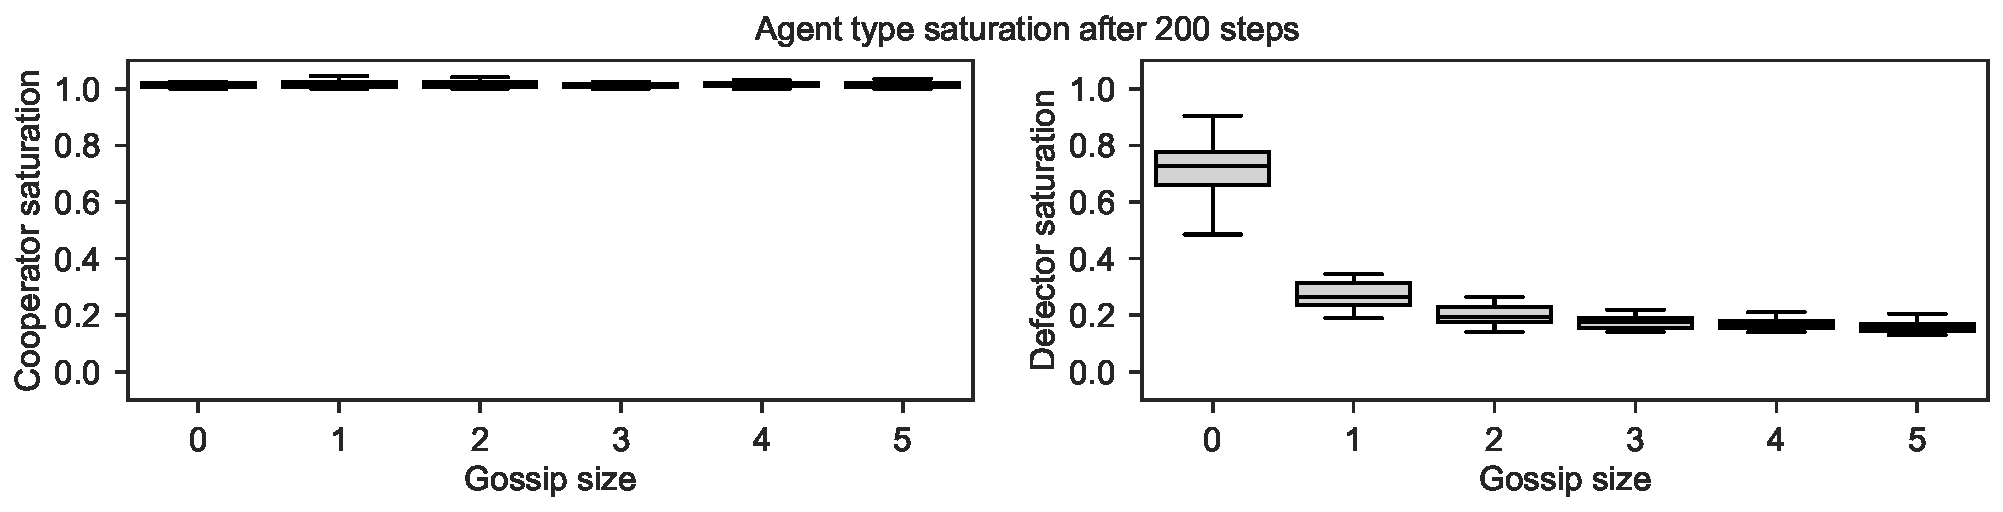
\includegraphics[width=\paperwidth-4cm]{saturation&gossip_size-range1_200steps_large.pdf}
  }
  \makebox[\textwidth]{
    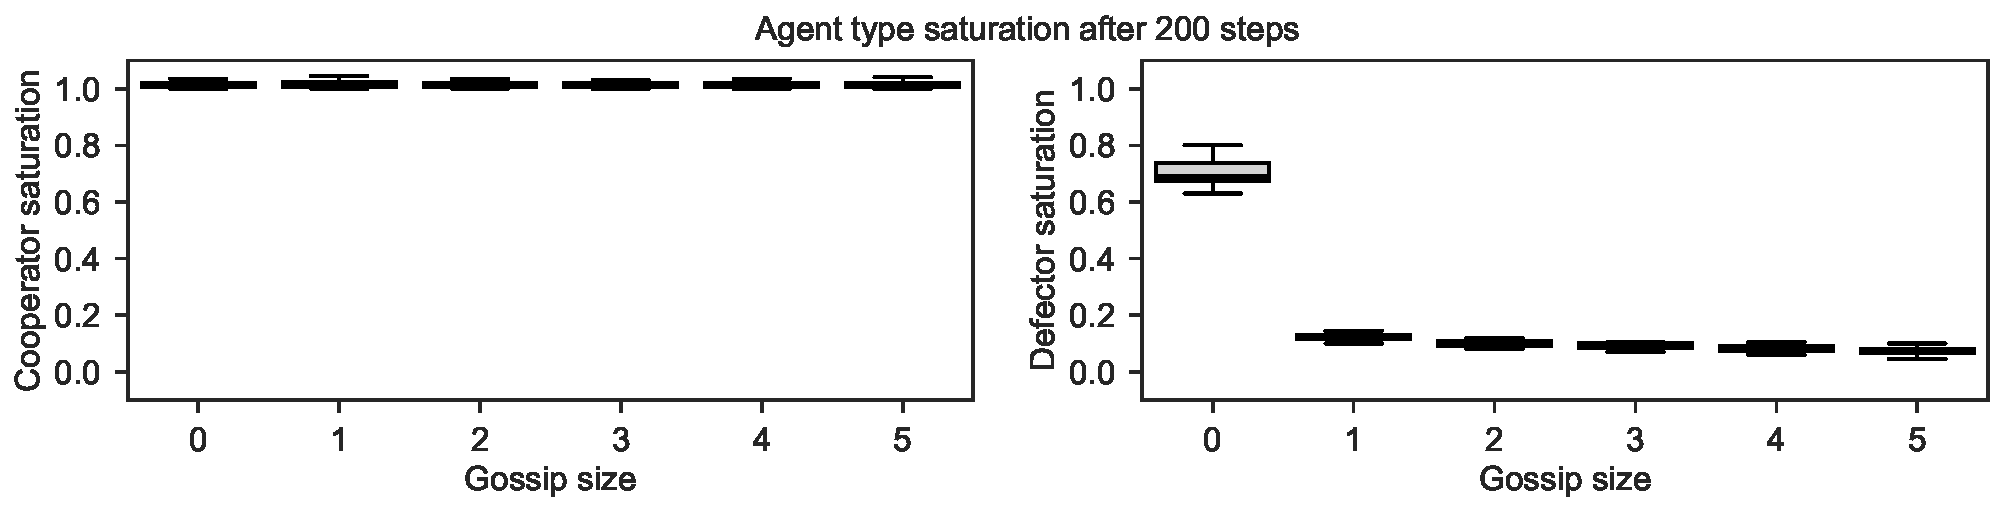
\includegraphics[width=\paperwidth-4cm]{saturation&gossip_size-range2_200steps_large.pdf}
  }
  \makebox[\textwidth]{
    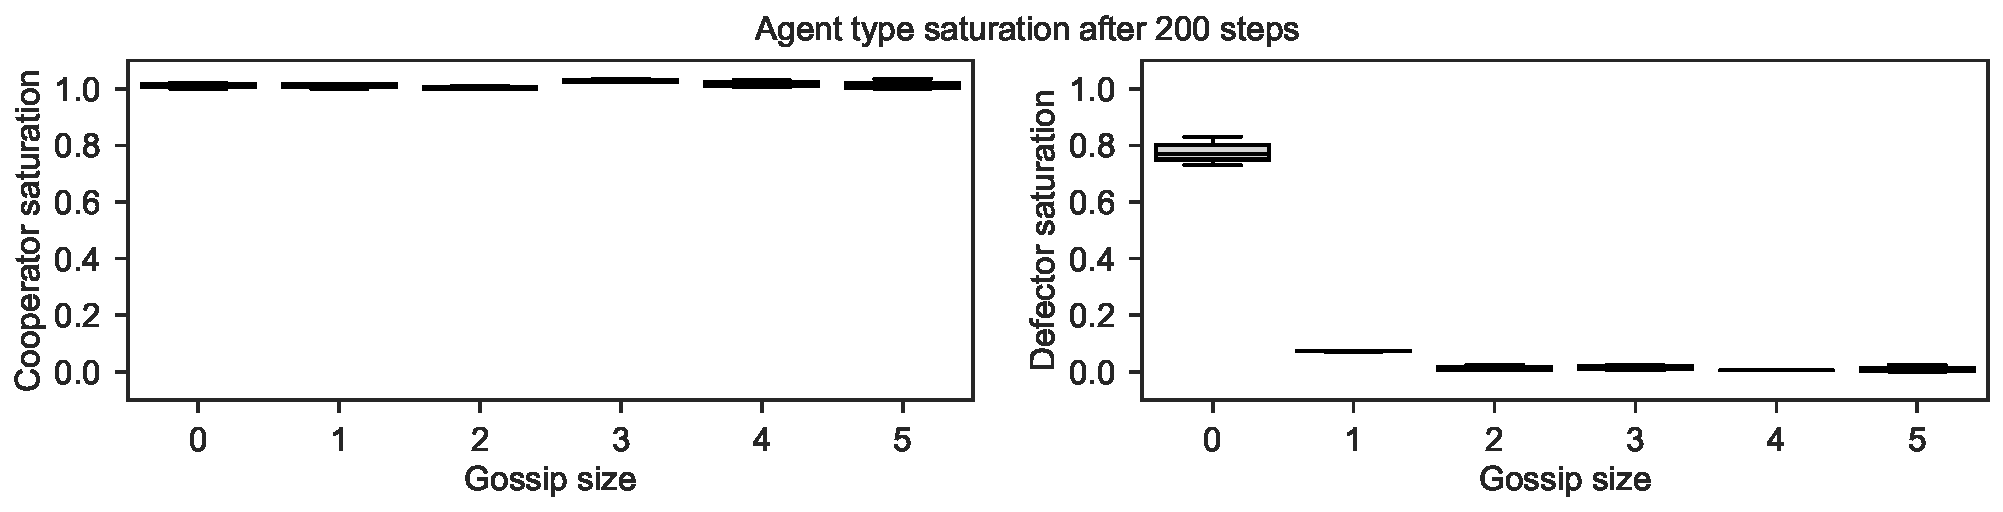
\includegraphics[width=\paperwidth-4cm]{saturation&gossip_size-range3_200steps_large.pdf}
  }
  \caption{Agent type saturation for various gossip sizes after 200 steps, gossip radii 1, 2, and 3, respectively top to bottom; SD of 30 simulation runs, outliers removed}
  \label{fig:agent_sat/gossip_size_step200}
\end{figure}

\begin{figure}[!h]
  \centering
  \makebox[\textwidth]{
    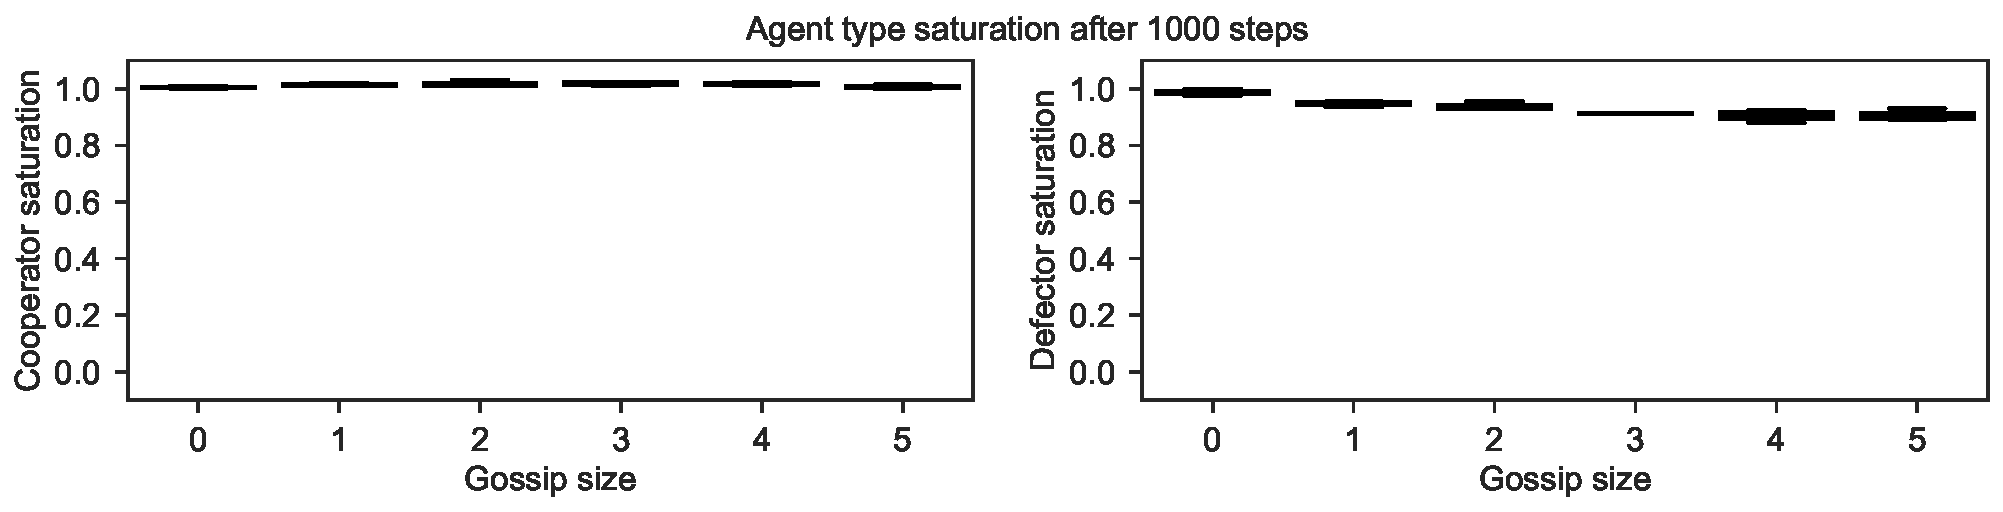
\includegraphics[width=\paperwidth-4cm]{saturation&gossip_size-range1_1000steps_large.pdf}
  }
  \makebox[\textwidth]{
    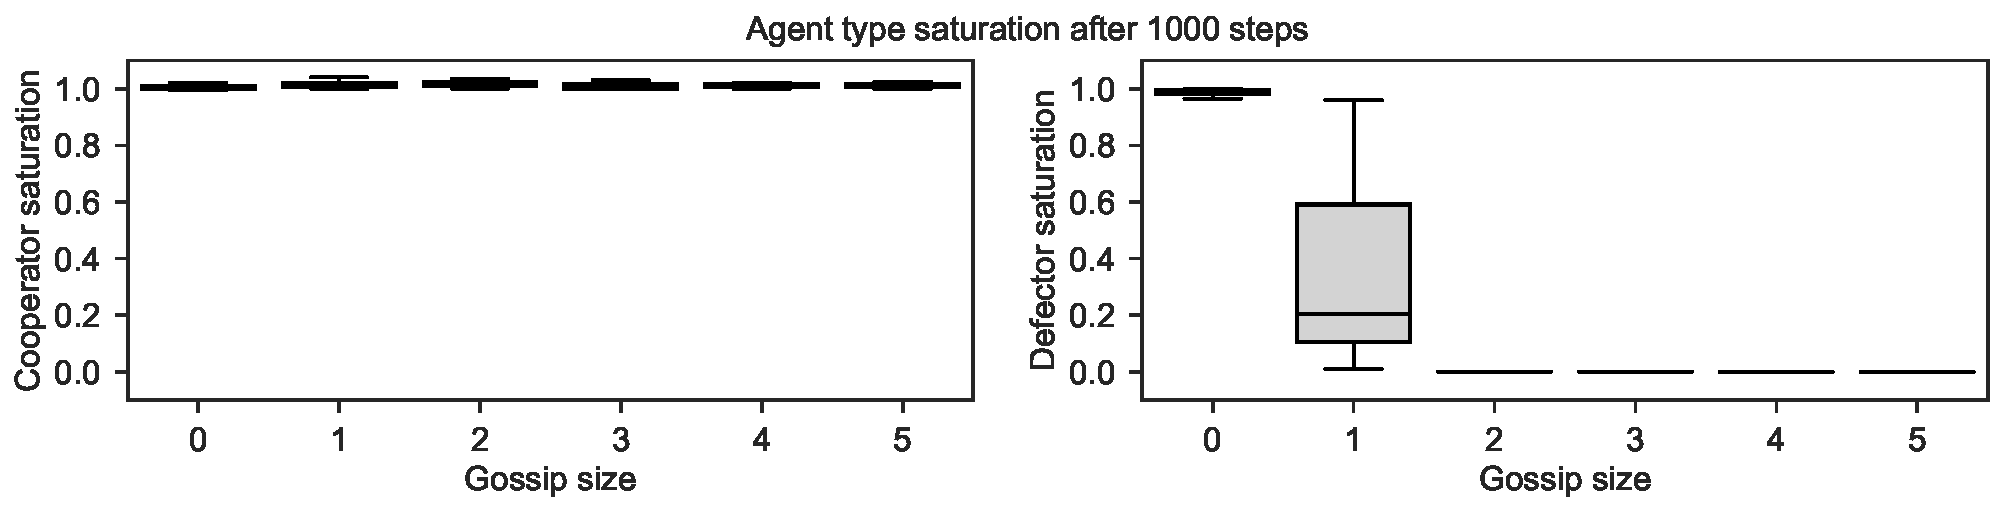
\includegraphics[width=\paperwidth-4cm]{saturation&gossip_size-range2_1000steps_large.pdf}
  }
  \makebox[\textwidth]{
    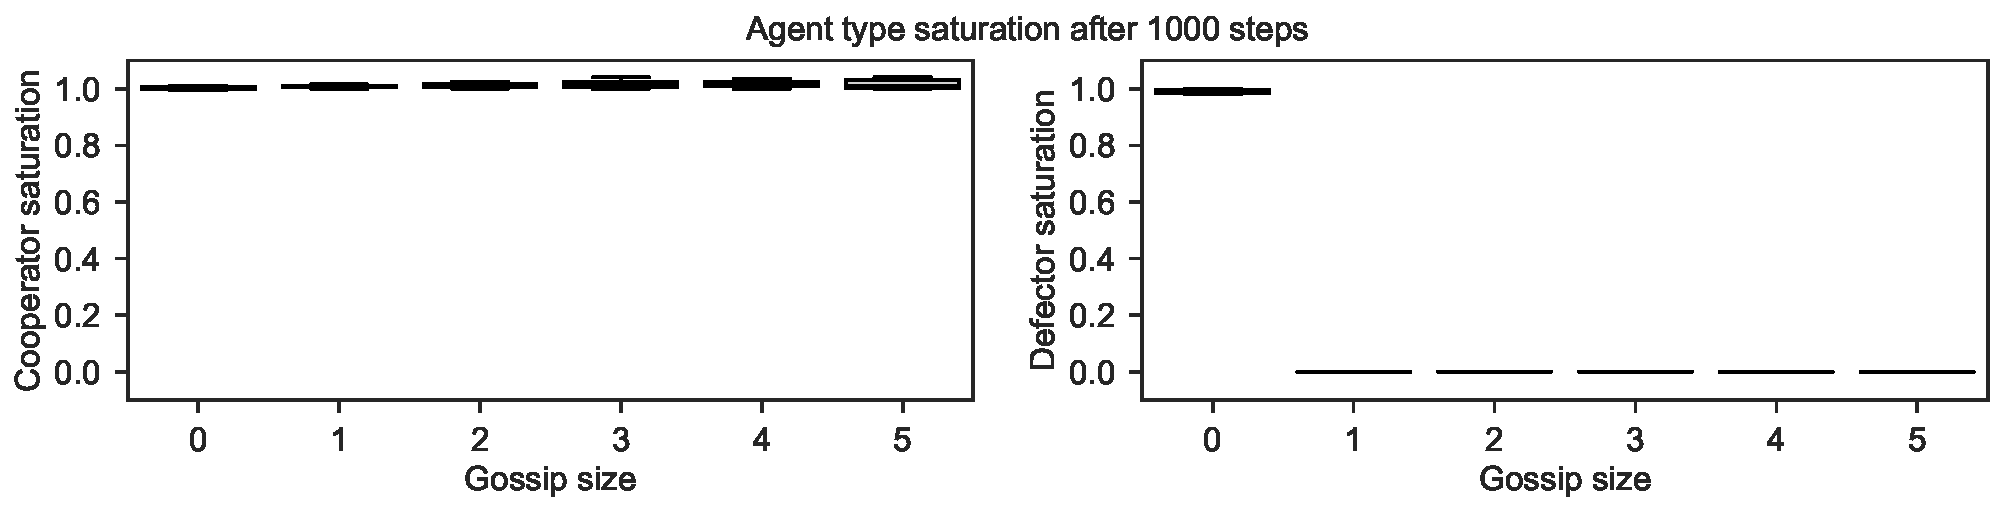
\includegraphics[width=\paperwidth-4cm]{saturation&gossip_size-range3_1000steps_large.pdf}
  }
  \caption{Agent type saturation for various gossip sizes after 1000 steps, gossip radii 1, 2, and 3, respectively top to bottom; SD of 30 simulation runs, outliers removed}
  \label{fig:agent_sat/gossip_size_step1000}
\end{figure}

We have found that the introduction of gossip is a strong deterrent of defection and leads to cooperator-only populations quickly.
The size of the memory and the size of the gossip are not significant factors, only speeding up the convergence slightly.
The most important factor in predicting cooperator success is the range of the gossip.


\subsection{Robustness of the gossip}
To check the effectiveness and robustness of our model against environmental harshness we will
use the same simulation setup for determining the $S$ value from the beginning of this section (baseline model).
We will plot agent type saturations across various $S$ (sucker's payoff).

To test the gossip model at the extreme, we will use memory size of 1, gossip size of 1 and gossip range of 3.
We will run the simulation for 250 and 1000 steps.
The final agent type saturations are plotted in Figure \ref{fig:agent_sat/S_final}.

\begin{figure}[!h]
  \centering
  \makebox[\textwidth]{
    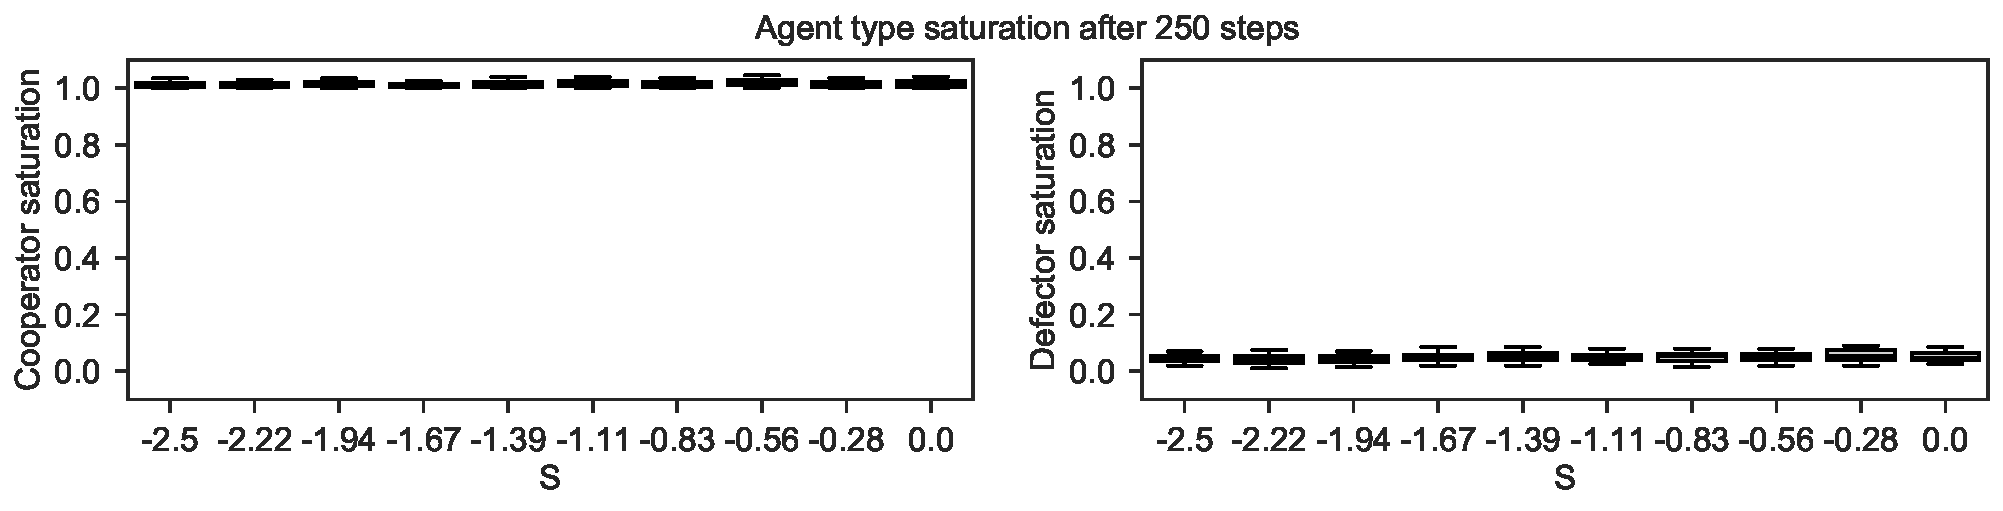
\includegraphics[width=\paperwidth-4cm]{saturation&S-memory1_gossip1_range3_250steps_large.pdf}
  }
  \makebox[\textwidth]{
    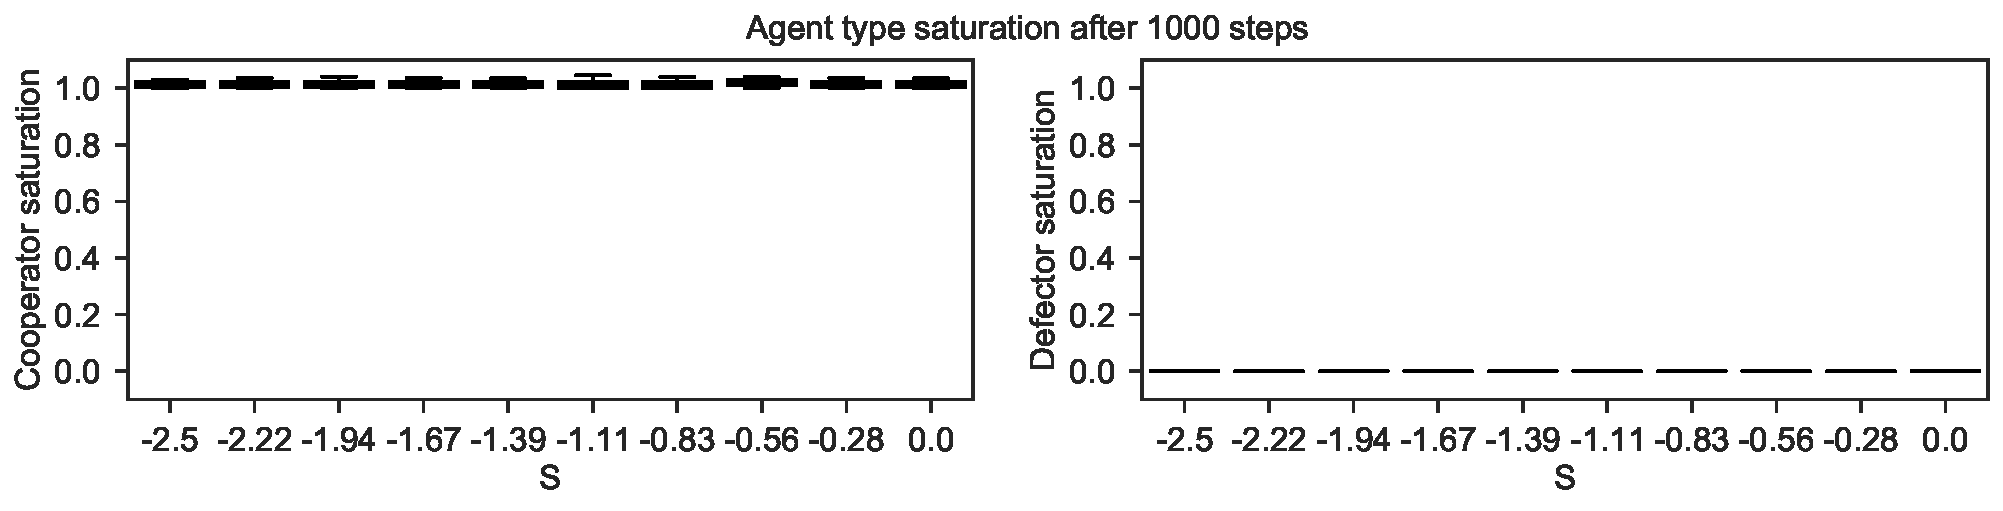
\includegraphics[width=\paperwidth-4cm]{saturation&S-memory1_gossip1_range3_1000steps_large.pdf}
  }
  \caption{Agent type saturation for various $S$ (sucker's payoff) after 250 and 1000 steps, memory size 1, gossip size 1, gossip range 3; SD of 30 simulation runs, outliers removed}
  \label{fig:agent_sat/S_final}
\end{figure}

Next we fix $S = -1.5$ again and vary the cost of living $0.0 \leq k \leq 3.5$ instead.
In Figure \ref{fig:agent_sat/k_final} we plot the achieved saturations.
With $3.0 \leq k$, which means $R \leq k$, we see that all agents go extinct.
Another interesting case is $k = 0.0$, meaning no cost of living is imposed on the agents,
there is no counter pressure on the defectors, so they are able to survive; cooperators also manage to reach and sustain fully saturated population.
For all values between these extremes the gossip model (with range 3) enforces cooperator-only population.

\begin{figure}[!h]
  \centering
  \makebox[\textwidth]{
    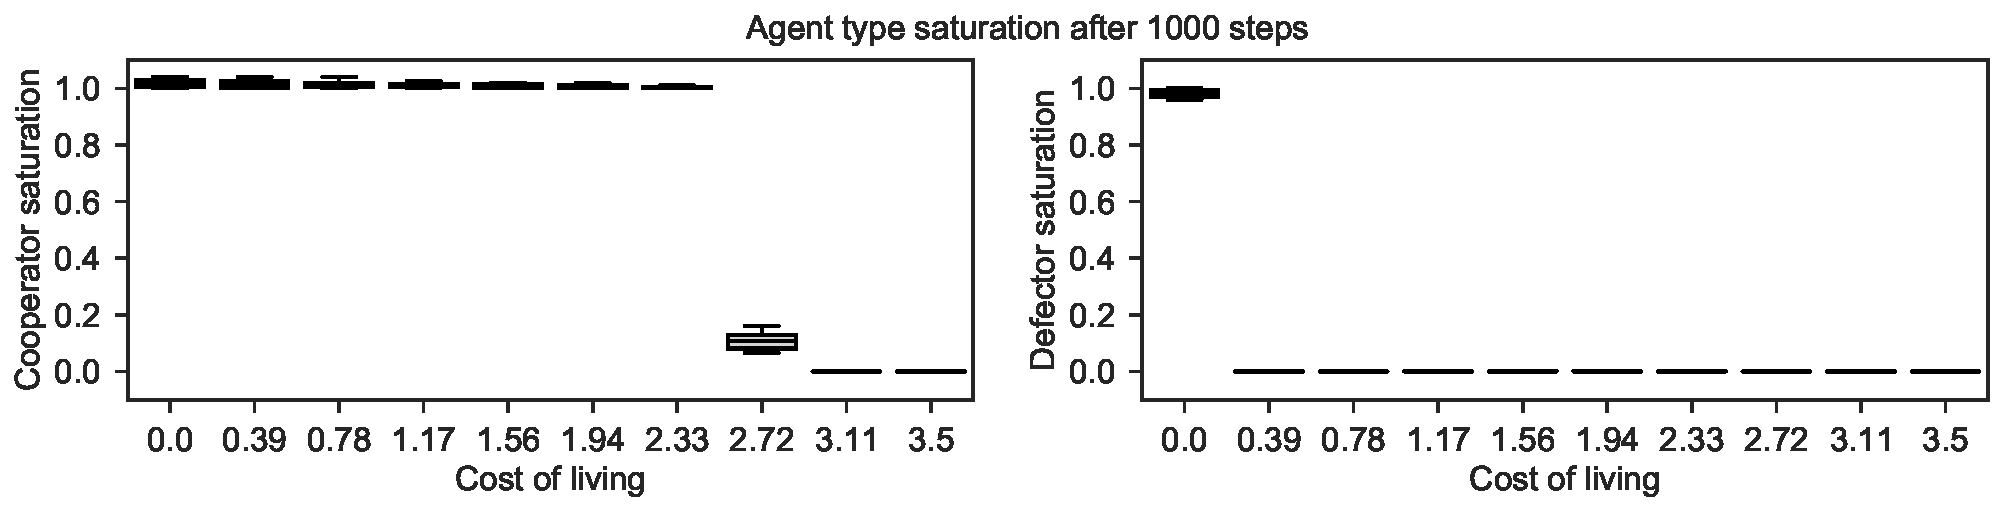
\includegraphics[width=\paperwidth-4cm]{saturation&living_cost-memory1_gossip1_range3_1000steps_large.pdf}
  }
  \caption{Agent type saturation for various $k$ (cost of living) after 1000 steps, memory size 1, gossip size 1, gossip range 3; SD of 30 simulation runs, outliers removed}
  \label{fig:agent_sat/k_final}
\end{figure}


\subsection{Spatial patterns}

\begin{figure}[!hb]
  \centering
  \textbf{Baseline:} Memory size 0 - Gossip size 0 - Gossip range 0
  \makebox[\textwidth]{
    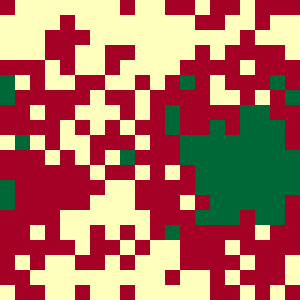
\includegraphics[width=\textwidth/4]{spatial-memory0+gossip0+range0.pdf}
    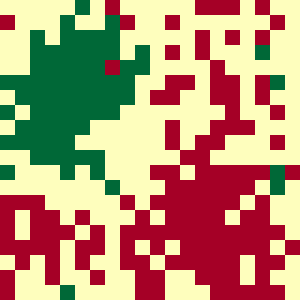
\includegraphics[width=\textwidth/4]{spatial-memory0+gossip0+range0-B.pdf}
    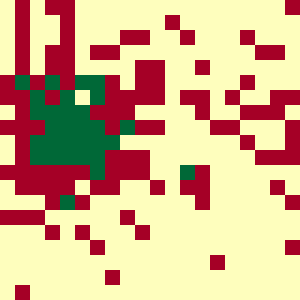
\includegraphics[width=\textwidth/4]{spatial-memory0+gossip0+range0-C.pdf}
  }
  \textbf{Memory-5:} Memory size 5 - Gossip size 0 - Gossip range 0
  \makebox[\textwidth]{
    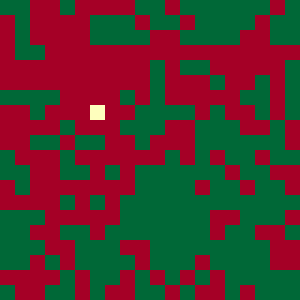
\includegraphics[width=\textwidth/4]{spatial-memory5+gossip0+range0-A.pdf}
    
\includegraphics[width=\textwidth/4]{spatial-memory5+gossip0+range0-B.pdf}
    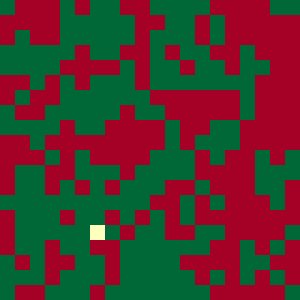
\includegraphics[width=\textwidth/4]{spatial-memory5+gossip0+range0-C.pdf}
  }
  \textbf{Final:} Memory size 1 - Gossip size 1 - Gossip range 3
  \makebox[\textwidth]{
    
\includegraphics[width=\textwidth/4]{spatial-memory1+gossip1+range3-A.pdf}
    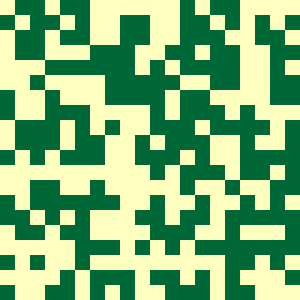
\includegraphics[width=\textwidth/4]{spatial-memory1+gossip1+range3-B.pdf}
    
\includegraphics[width=\textwidth/4]{spatial-memory1+gossip1+range3-C.pdf}
  }
  \caption{Spatial patterns formed by agents after simulating for 500 steps, defectors are red, cooperators are green}
  \label{fig:spatial}
\end{figure}

We include images of the spatial patterns formed by the simulations in Figure \ref{fig:spatial}.
Since the model has an inspiration in biology this is an interesting visualization to include.
We show 3 patterns formed after simulating for 500 steps for each of the following configurations
(these are the same as used in the sections above):
\begin{enumerate}
  \setlength\itemsep{0em}
  \setlength\parskip{0cm}
  \item
    \textbf{Baseline:} the base model, without any extensions (0-memory, no gossip)
  \item
    \textbf{Memory-5:} every agent can remember the 5 most recently encountered defectors
  \item
    \textbf{Final:} every agent can remember the single last defector and gossip about it,
    radius of the gossip is 3 units in a Moore neighborhood
\end{enumerate}



\section{Discussion}
% Results can be compared to known results and placed in a broader context.
% Provide a reflection on what has been concluded and how this was done.
% Then give a further possible explanation of results.

Looking back at the results we collected in the previous section;
now we present a more in-depth commentary on their meaning and
put them in a wider context.

We have seen that the baseline model act as expected and leads to total extinction quickly.
This is consistent with the behaviour observed by \citet{smaldino}.
Agents can prolong their existence if the cooperators are able to form a cluster,
but there is no escaping eventual extinction.

By extending the model with memory, we are able to sustain the population.
Both cooperators and defectors profit from this equally, with cooperators having a slight edge
as memory size increases - although this is almost negligible.
In the spatial patterns for the memory-5 model we see more fragmentation: this is because cooperator can survive next to defectors by remembering them.

From \citet{simple-reputation, public-private-monitoring} we know that reputation systems promote cooperation.
We wanted to see if local reputation system suffices: we let agents communicate what they remember to nearby agents.
This works very well, we can consistently achieve cooperator-only population quickly.
The amount of the information included in the gossip is not very important, the main parameter is the range of the gossip. By increasing it we can converge to cooperation faster.

Last we looked at the robustness of the local reputation model against environmental harshness.
We found it to be almost entirely independent of the environmental parameters.
The gossip mechanism is too strong to be influenced by environmental effects.
We conclude by certifying the efficacy of the local reputation, confirming our hypotheses.



\section{Responsible Research}
We recognize the inherent difficulties in conducting ethical and sustainable research.
We take the following actions to ensure this paper is ethically good and can be reproduced by others.

We want to make this paper a good foundation for future work and as such we provide all source materials for this paper: including the code files for running the simulations and evaluating results, the \LaTeX\ files for this paper, and anything else used while conducting this research.
Next, we use Nix Flake\footnote{\url{https://nixos.wiki/wiki/Flakes}} to capture the exact versions of all software, libraries, and packages used for this research \citep{nix}. All of this is captured together in and provided as a fully reproducible environment.
We hope that by doing this it becomes easy to reproduce our results and provide a good foundation environment for other researchers to quickly kick-start their research.
Our model itself is implemented in a Jupyter Notebook\footnote{\url{https://jupyter.org/}} and care was taken to keep the total amount of dependencies as low as possible and to stick to the most standard dependencies wherever possible.
We hope others will appreciate this by building upon our research and uncovering wonderful conclusions.

This paper explores the effects of reputation on promoting and sustaining cooperation.
We believe this research is ethically good and our conscience is clean about the methods used and conclusions reached; as well as all other aspects of this paper.
While we cannot ensure the findings of this paper will not be misused by others, we implore all readers to always strive for the highest ethical ideals.
Let's all be excellent.




\section{Conclusion}
% ideally, this section can stand on its own: it should be readable without having read the earlier sections.
In this paper, we wanted to investigate the efficacy of gossip in disseminating local reputation, promoting and sustaining cooperation in a population of rational selfish agents acting independently.

Cooperation is the single best advantage humans have over other species;
it is shown over and over again that cooperating individuals can achieve extraordinary results and reap astronomical rewards.
Yet, the conditions necessary and sufficient for cooperation to emerge and sustain itself are not well known or understood.
We find it important to investigate what makes cooperation the preferred strategy and how to promote it in diverse populations.

We have built a computer simulation of a multi-agent spatial environment.
The main agent interaction was modelled using a Prisoner's Dilemma exchange game. This is a well understood game with lots of game theory research shedding light on its various interactions.
We have based our model on the work of \citet{smaldino}, with a couple of changes to better fit our goal.
Namely, we have decreased the grid size to keep the simulation times reasonably low.
This has led us to change the PD game reward $S$ (sucker's payoff) to compensate for the smaller amount of agents in the new model.

We have expanded the model with memory; each agent can remember a fixed number of past defectors and choose to abstain from playing games with them, thus protecting itself against being exploited repeatedly.
We found that adding memory to the model made cooperators fully saturate the population quickly, but the defectors would catch up shortly afterwards.
Increasing memory size beyond one brought only marginal benefits in increasing the saturation speed.

Next, we have allowed the agents to communicate. Before playing a game with a nearby opponent, an agent can ask all agents in a range if they remember the opponent as a defector. If they do, the agent will abstain from playing the game with the opponent.
Thus a single defection can be punished by being effectively barred from all future interactions with other agents.
This ostracization quickly leads to death, since agents are not able to survive without a steady stream of rewards from the PD game.
By allowing agents to gossip openly, cooperators were able to avoid exploitation. Defectors die out quickly.
The amount of gossip information was not an important factor, again only bringing a negligible increase in the saturation speed.

The most important factor in predicting cooperator success is the range at which the gossip can be exchanged.
If the gossip can move faster than agents, cooperators will flourish.  Otherwise defectors can reach full population saturation.
From what we find, the best way to ensure cooperation (and survival of a population) is to keep your enemies close and be loud about it.
The louder the better.

Our model and simulation setup was limited in representing real world conditions.
We assume all information is transferred with 100\% fidelity - no noise is present, no information is lost, all agents share information willingly and openly with anyone without any limitations. Introduction of noise to this model could alter the results and show other interesting aspects of cooperation.

Next, the size of spatial environment was kept very small because of constrained computation resources. Expanding the grid size would allow for more complex interactions and long-memory effects between the agents.
It would be interesting to investigate if expanding the grid size alters the results in any meaningful way.

The population of agents we have used was composed of pure cooperators and pure defectors.
And all agents were sharing information openly with anyone.
More complex strategies could be defined and perhaps an optimal strategy for behaviour/information sharing could be found.

Agents could be given probabilistic behaviour. Making the classification into cooperator/defector more complex. This would work against the gossip mechanism we used.
It could be possible that the gossip mechanism would not be advantageous if the agent behaviour was random enough.
Perhaps even favoring the defectors as the gossip mechanism would deter more cooperator-cooperator interactions.

Our simulation setup is available
(\url{https://github.com/tinybeachthor/IPD})
for anyone interested in investigating any of these or other effects.



\pagebreak
\bibliography{references}

\end{document}
